\chapter{Thin two-level graphs}
\label{chap:twolevel}

Breu \cite{breuAlgorithmicAspectsConstrained1996} has presented in his thesis a similar class of constrained unit disk graphs where the disks are placed on $k$ horizontal parallel lines. More formally: a disk $(x,y)$ can be placed in $x \in (-\infty,\infty)$ and $y \in L$ with $|L| = k$.

In this chapter I define thin two-level graphs as a two-level graph where $L = \{0,\epsilon\}$ and $\epsilon$ is an arbitrarily small real number.


\section{Characterization of TTL}

\prop {An $\sigma$-SG($c$) graph $G$ (with $c < 1$) can be characterized by computing $\delta : A \times B \to E$ where $A,B \subseteq G$, $A$ and $B$ are UIG, and $A \cup B = \varnothing$:

\[
    \delta(x,y) =
    \begin{cases}
      xy        & \text{if } \text{dist}(x,y) \leq 1\\
      \varnothing,       & \text{otherwise}
    \end{cases}
\]
}
\todo{this proposition is ugly, re-do this with Breu's notations.}

\begin{figure}
\centering

\begin{scaletikzpicturetowidth}{\textwidth}
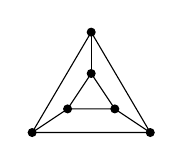
\begin{tikzpicture}[scale=1.5]

%graph
\node[draw,circle,inner sep=1pt,fill,label distance=1cm] (v2) at (0,0.85) {};
\node[draw,circle,inner sep=1pt,fill,label distance=1cm] (v2) at (-0.5,0) {};
\node[draw,circle,inner sep=1pt,fill,label distance=1cm] (v2) at (0.5,0) {};
\draw(0.5,0)--(-0.5,0)--(0,0.85)--(0.5,0);

\node[draw,circle,inner sep=1pt,fill,label distance=1cm] (v2) at (0,0.5) {};
\node[draw,circle,inner sep=1pt,fill,label distance=1cm] (v2) at (0.2,0.2) {};
\node[draw,circle,inner sep=1pt,fill,label distance=1cm] (v2) at (-0.2,0.2) {};
\draw(0,0.5)--(0.2,0.2)--(0.2,0.2)--(-0.2,0.2)--(0,0.5);

\draw(0,0.5)--(0,0.85);
\draw(-0.5,0)--(-0.2,0.2);
\draw(0.2,0.2)--(0.5,0);


\end{tikzpicture}
\end{scaletikzpicturetowidth}

\caption{ Forbidden graph in TTL }
\label{fig:forbSigma}
\end{figure}

This class of graphs is close to our main class TSG. But we have to know at what point we can rely in this class of graphs to study TSG:

\lemma[Breu \cite{breuAlgorithmicAspectsConstrained1996}]{
  \label{lemma:chordlessLEVEL}
  Let $abcda$ be a chordless 4-cycle in a two-level graph $G=(V,E)$. Then $ad$ and $bc$ are level edges (they are adjacent in the same level), and the others are cross edges for every realization $\phi$ of $G$ for which $\phi(a)_x<\phi(c)_x$ and $\phi(b)_x<\phi(d)_x$.
}


With this preliminary result, we proceed to one of our main results:

\theorem{TTL $\subsetneq$ TSG}

\proof{By definition, we know that TTL $\subset$ TSG because the area where the disks can be placed in TTL is included in the area in TSG.

We can prove that TTL $\neq$ TSG because we can construct a graph $G$ such that $G \in$ TSG and $G \notin$ TTL. This graph $D$ is a net$^*$ graph as described in Figure \ref{fig:forbSigma}.
\begin{proofpart}
  $D$ is a TSG because we can realize it as a TSG if we take as center of disks $(0,0)$, $(0,z)$, $(0,\epsilon)$, $(1,0)$, $(1,z)$, $(1,\epsilon)$ such that $0 < z < \epsilon$.
\end{proofpart}
\begin{proofpart}
  Now we have to prove that $D$ is a forbidden induced subgraph of TTL. We will try to construct it by taking a induced subgraph that is realizable: we take $D_{-1} = D - x$ with $x\in V(D)$. We notice that $V(D_{-1})$ is a chordless $C_{4}$ ($abcd$) with a vertex $e$ adjacent to any two consecutive vertices $x,y \in V(C_4)$ creating the triangle $xye$.

  By Lemma \ref{lemma:chordlessLEVEL} we know that $abcda$ is a cycle if $ab$ and $cd$ are level edges. We can classify these vertices in two sets: $\ell(V) = {a,d}$ and $r(V) = {b,c}$ where $\forall u\in \ell(V) v\in r(V): \phi(u)_x < \phi(v)_x$.

  To realize $D_{-1}$ we have to add a vertex $e$ to $C_4$. In our case, $e$ cannot be added in two
  \todo{Finish proof here}
\end{proofpart}
}

\subsection{Relation with MUIG}

A big question that was asked during this research is: What is the relationship between TTL and MUIG? We know that the net*-graph is forbidden for every two-level graph, this graph is also forbidden for MUIG because it includes an induced $C_4$; we can also see that every forbidden induced subgraph for MUIG also is for TTL.

However, $C_4$ is realizable for two-level graphs with $c = 1$ in general, which means TTL $\neq$ interval $=$ MUIG. We then know that TTL $\cup$ MUIG $\subseteq$ TSG with TTL $\neq$ MUIG.

\todo[inline]{Rewrite this better.}

\section{Induced forbidden subgraphs}

\begin{figure}
\centering

\begin{scaletikzpicturetowidth}{\textwidth}
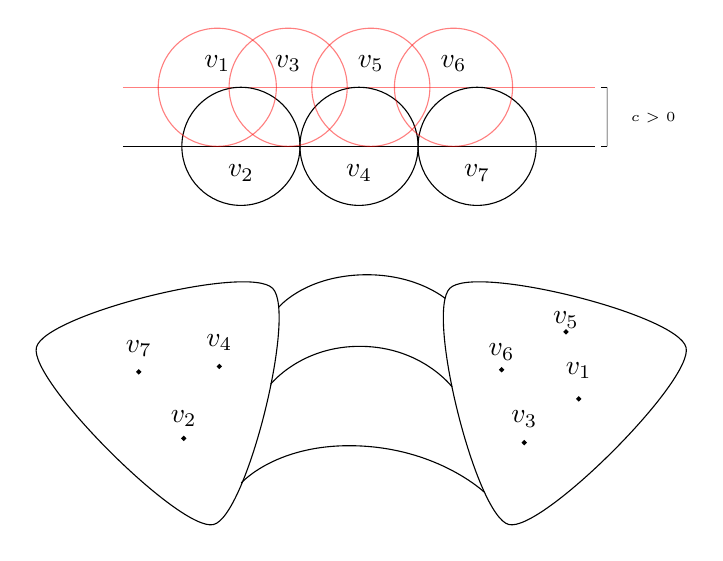
\begin{tikzpicture}[scale=1.5]
\draw (-2,0) -- (2,0);
\draw[red ,opacity = 0.5] (-2,0.5) -- (2,0.5);

\draw  (-1,0) circle [radius=0.5];
\draw[color=black] (-1,-0.2265) node {$v_2$};
\draw  (0,0) circle [radius=0.5];
\draw[color=black] (0,-0.2265) node {$v_4$};
\draw  (1,0) circle [radius=0.5];
\draw[color=black] (1,-0.2265) node {$v_7$};

\draw[red, opacity = 0.5] (0.1,0.5) circle [radius=0.5];
\draw[color=black] (0.1,0.7) node {$v_5$};
\draw[red, opacity = 0.5] (0.8,0.5) circle [radius=0.5];
\draw[color=black] (0.8,0.7) node {$v_6$};
\draw[red, opacity = 0.5] (-0.6,0.5) circle [radius=0.5];
\draw[color=black] (-0.6,0.7) node {$v_3$};
\draw[red, opacity = 0.5] (-1.2,0.5) circle [radius=0.5];
\draw[color=black] (-1.2,0.7) node {$v_1$};
\draw[color=black] (2.4902,0.2393) node {\tiny $c > 0$};

% lines to describe distance (epsilon)
\draw[very thin] (2.1003,0.5) -- (2.1,0);
\draw[very thin] (2.0489,0.5) -- (2.0997,0.5);
\draw[very thin] (2.05,0) -- (2.1,0);

%graph
\draw plot [smooth cycle] coordinates {(-1.2314,-3.2019) (-2.7314,-1.7019) (-0.7314,-1.2019) } ;
\draw plot [smooth cycle] coordinates {(1.2686,-3.2019) (0.7686,-1.2019) (2.7686,-1.7019) } ;


\node[draw,circle,inner sep=0.5pt,fill,label distance=1cm] (v2) at (-1.4847,-2.4724) {};
\draw[color=black] (-1.4847,-2.3019) node {$v_2$};
\node[draw,circle,inner sep=0.5pt,fill,label distance=1cm] (v2) at (-1.1831,-1.8637) {};
\draw[color=black] (-1.1831,-1.6637) node {$v_4$};
\node[draw,circle,inner sep=0.5pt,fill,label distance=1cm] (v2) at (-1.8649,-1.9094) {};
\draw[color=black] (-1.8649,-1.7094) node {$v_7$};

\draw plot [smooth,tension=1.2] coordinates {(-0.6778,-1.3597) (-0.0024,-1.0888)(0.7295,-1.288)} node at (1,0) {};
\draw plot [smooth,tension=1.2] coordinates {(-0.9968,-2.8499) (-0.0099,-2.5359)(1.0588,-2.9266)} node at (1,0){};
\draw plot [smooth,tension=1.2] coordinates {(-0.7488,-2.0147) (0.0223,-1.6933)(0.7878,-2.0368)} node at (1,0){};

\node[draw,circle,inner sep=0.5pt,fill,label distance=1cm] (v2) at (1.86,-2.1379) {};
\draw[color=black] (1.86,-1.8979) node {$v_1$};
\node[draw,circle,inner sep=0.5pt,fill,label distance=1cm] (v2) at (1.399,-2.509) {};
\draw[color=black] (1.399,-2.309) node {$v_3$};
\node[draw,circle,inner sep=0.5pt,fill,label distance=1cm] (v2) at (1.7518,-1.5712) {};
\draw[color=black] (1.7518,-1.4712) node {$v_5$};
\node[draw,circle,inner sep=0.5pt,fill,label distance=1cm] (v2) at (1.2071,-1.8911) {};
\draw[color=black] (1.2071,-1.7411) node {$v_6$};

\end{tikzpicture}
\end{scaletikzpicturetowidth}

\caption{ A representation of a TL($c$) }
\label{fig:sigma}
\end{figure}
